% !TEX program = xelatex
\documentclass[10pt,letterpaper,twocolumn]{article}

\usepackage[top=0.72in,bottom=0.72in,left=0.72in,right=0.72in]{geometry}
\usepackage{fontspec}
\setmainfont{Latin Modern Roman}[
  Extension=.otf,UprightFont=lmroman10-regular,BoldFont=lmroman10-bold,
  ItalicFont=lmroman10-italic,BoldItalicFont=lmroman10-bolditalic]
\setsansfont{Latin Modern Sans}[
  Extension=.otf,UprightFont=lmsans10-regular,BoldFont=lmsans10-bold,
  ItalicFont=lmsans10-oblique,BoldItalicFont=lmsans10-boldoblique]
\setmonofont{Latin Modern Mono}[Extension=.otf,UprightFont=lmmono10-regular,Scale=0.82]
\newfontfamily\acbold{ywft-processing-bold}[
  Path=../../system/public/type/webfonts/,Extension=.ttf]
\newfontfamily\aclight{ywft-processing-light}[
  Path=../../system/public/type/webfonts/,Extension=.ttf]

\usepackage{xcolor}
\usepackage{titlesec}
\usepackage{enumitem}
\usepackage{booktabs}
\usepackage{tabularx}
\usepackage{fancyhdr}
\usepackage{hyperref}
\usepackage{xurl}
\usepackage{graphicx}
\usepackage{microtype}
\usepackage{listings}
\usepackage[numbers,sort&compress]{natbib}
\usepackage{tikz}
\usetikzlibrary{arrows.meta,positioning,fit}

\definecolor{acpink}{RGB}{180,72,135}
\definecolor{acblue}{RGB}{44,92,188}
\definecolor{acred}{RGB}{190,48,62}
\definecolor{acdark}{RGB}{48,43,56}
\definecolor{acgray}{RGB}{105,105,110}
\definecolor{aclightgray}{RGB}{244,243,246}

\hypersetup{colorlinks=true,linkcolor=acblue,urlcolor=acblue,citecolor=acblue,
  pdfauthor={@jeffrey},
  pdftitle={OSKIEWAR: A Cross-Platform Fighting-Game Laboratory for Aesthetic Computer}}
\titleformat{\section}{\normalfont\bfseries\normalsize\uppercase}{\thesection.}{0.45em}{}
\titlespacing{\section}{0pt}{1.15em}{0.3em}
\titleformat{\subsection}{\normalfont\bfseries\small}{\thesubsection}{0.45em}{}
\titlespacing{\subsection}{0pt}{0.8em}{0.2em}
\pagestyle{fancy}
\fancyhf{}
\renewcommand{\headrulewidth}{0pt}
\fancyhead[C]{\footnotesize\color{acpink}\textit{OSKIEWAR --- system report}}
\fancyfoot[C]{\footnotesize\thepage}
\setlist[itemize]{nosep,leftmargin=1.2em,itemsep=0.1em}
\setlength{\columnsep}{1.7em}
\setlength{\parindent}{1em}
\setlength{\parskip}{0.25em}
\makeatletter
\setlength{\@fptop}{0pt}
\setlength{\@dblfptop}{0pt}
\makeatother
\tolerance=900
\emergencystretch=1em
\graphicspath{{../arxiv-ac/figures/}}
\newcommand{\ac}{\textsc{Aesthetic.Computer}}
\newcommand{\game}{\textsc{OSKIEWAR}}
\newcommand{\code}[1]{\texttt{#1}}
\InputIfFileExists{version.tex}{}{%
  \providecommand{\paperhash}{dev}\providecommand{\paperrev}{?}}

\lstset{basicstyle=\ttfamily\footnotesize,breaklines=true,frame=single,
  rulecolor=\color{acgray!30},backgroundcolor=\color{aclightgray},
  xleftmargin=0.4em,xrightmargin=0.4em,aboveskip=0.5em,belowskip=0.5em}

\begin{document}

\twocolumn[{%
\begin{center}

\includegraphics[height=3.5em]{pals}\par\vspace{0.45em}
{\acbold\fontsize{23pt}{27pt}\selectfont\color{acdark} OSKIEWAR}\par
\vspace{0.2em}
{\aclight\fontsize{12pt}{14pt}\selectfont\color{acpink}
  A Cross-Platform Fighting-Game Laboratory for Aesthetic Computer}\par
\vspace{0.55em}
{\normalsize\href{https://prompt.ac/@jeffrey}{@jeffrey}}\par
{\small\color{acgray} Aesthetic.Computer --- 4 August 2026}\par
{\small\color{acgray} ORCID: \href{https://orcid.org/0009-0007-4460-4913}{0009-0007-4460-4913}}\par
\vspace{0.35em}
{\small\color{acblue}\url{https://aesthetic.computer}}\par
\vspace{0.55em}\rule{\textwidth}{1.5pt}\vspace{0.35em}
\end{center}

\begin{quote}
\small\noindent\textbf{Abstract.}
This paper records the first playable system build of \game{}, a two-player fighting-game laboratory whose complete client first ran as a native Universal Windows Platform application on Xbox and whose public spectator now runs as an Aesthetic Computer web piece. The game places Aesthetic Computer's URL-addressable program model inside a fixed-timestep 3D world rendered through an orthographic gameplay camera, with perspective cinematics for introductions and deaths. It combines quantized controller input, spatial sound, wind and ball physics, weapons, compact replays, browser spectation, and a low-latency OSC bridge for sound design in Ableton Live. The native host preserves a narrow capability boundary while the browser consumes a bounded, read-only match stream. Package 1.0.0.35, 49 automated client/relay/viewer checks, native preflight, browser rendering, and live telemetry support the implementation. The browser is not yet a feature-equivalent playable client; extracting simulation, pose, camera, and command mapping into platform-neutral modules is now the primary implementation direction.
\end{quote}
\vspace{0.4em}
}]

\section{From Controller Test to Game}

\game{} began as a request to put ``hello world'' on an Xbox and reveal each controller button as it was pressed. The test became a two-controller stick-figure arena: @jeffrey on player one, @oskie on player two, D-pad movement, up to jump, down to duck, and a quantized left stick so the analog device did not acquire a mechanically privileged move set. The working title was approved during play. Iteration then moved outward in three directions: a fighting system, a camera and world system, and a musical/network system.

The result remains a laboratory rather than a claim to a finished competitive fighter. Its useful property is that the whole loop is observable. Raw and quantized inputs, velocities, stances, hit regions, renderer timing, audio timing, and outbound signal transport can be surfaced while the match remains playable. This follows the Aesthetic Computer piece model---small programs with \code{boot}, \code{sim}, \code{paint}, \code{act}, and \code{leave} lifecycle functions---while extending the native host where console hardware requires explicit capabilities \cite{scudderPieces,scudderOS}. The web viewer returns the match to the ordinary URL-addressable piece system and establishes the first cross-platform seam.

\section{System Architecture}

The system has four layers (Figure~\ref{fig:architecture}). The Xbox shell owns Windows.Gaming.Input, rendering, audio, storage, HTTPS, UDP, and WebSocket transports. A QuickJS context runs \code{xbox/live/hello.js}. The script owns match rules and native presentation. A relay accepts latest-only spectator snapshots, the web piece renders them with the standard Aesthetic Computer lifecycle, and the monolith stores bounded replay demos. Ableton Live receives redundant OSC datagrams over the local network.

\begin{figure*}[t]
\centering
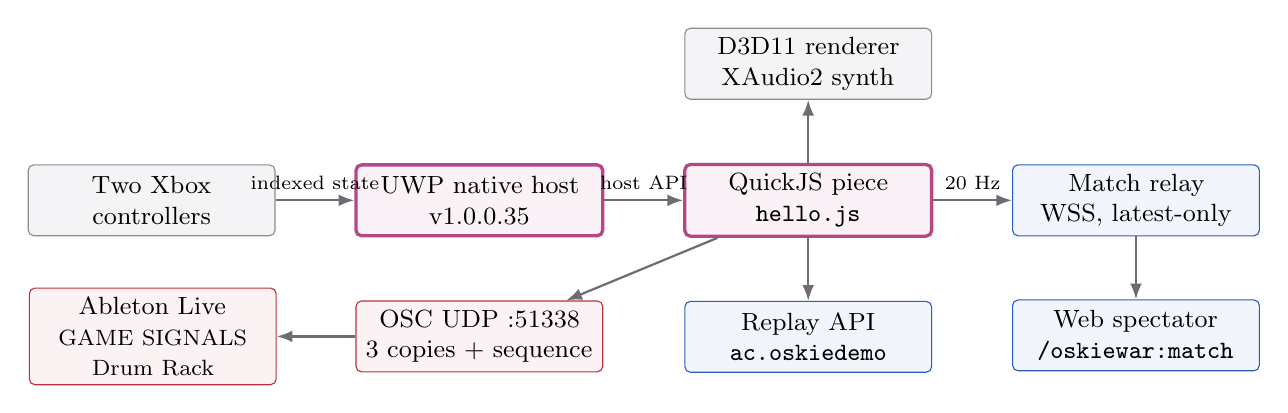
\begin{tikzpicture}[
  node distance=8mm and 10mm,
  box/.style={draw=acdark!55,rounded corners=2pt,fill=aclightgray,
    align=center,minimum height=9mm,text width=29mm,font=\small},
  core/.style={box,draw=acpink,very thick,fill=acpink!7},
  net/.style={box,draw=acblue,fill=acblue!6},
  audio/.style={box,draw=acred,fill=acred!6},
  arrow/.style={-{Latex[length=2mm]},thick,draw=acdark!70}]
  \node[box] (pads) {Two Xbox\\controllers};
  \node[core,right=of pads] (host) {UWP native host\\v1.0.0.35};
  \node[core,right=of host] (piece) {QuickJS piece\\\code{hello.js}};
  \node[box,above=of piece] (render) {D3D11 renderer\\XAudio2 synth};
  \node[net,right=of piece] (relay) {Match relay\\WSS, latest-only};
  \node[net,below=of relay] (phone) {Web spectator\\\code{/oskiewar:match}};
  \node[net,below=of piece] (replay) {Replay API\\\code{ac.oskiedemo}};
  \node[audio,below=of host] (osc) {OSC UDP :51338\\3 copies + sequence};
  \node[audio,left=of osc] (live) {Ableton Live\\{\footnotesize GAME SIGNALS}\\{\footnotesize Drum Rack}};
  \draw[arrow] (pads)--node[above,font=\scriptsize]{indexed state}(host);
  \draw[arrow] (host)--node[above,font=\scriptsize]{host API}(piece);
  \draw[arrow] (piece)--(render);
  \draw[arrow] (piece)--node[above,font=\scriptsize]{20 Hz}(relay);
  \draw[arrow] (relay)--(phone);
  \draw[arrow] (piece)--(replay);
  \draw[arrow] (piece)--(osc);
  \draw[arrow] (osc)--(live);
\end{tikzpicture}
\caption{The native shell owns privileged I/O; browser spectators receive bounded state through the relay and never connect to the console directly.}
\label{fig:architecture}
\end{figure*}

\subsection{Native capability boundary}

The host API exposes indexed \code{gamepad(0)} and \code{gamepad(1)} state, controller inventory, monotonic/unix clocks, timing and audio metrics, telemetry, drawing primitives, 3D triangles, textured sprites, Aesthetic Computer typefaces, oscillators, drums, and local persistence. Four purpose-built calls cross the machine boundary: \code{gameSignal(event,player,value,value2)}, \code{saveReplay(json)}, \code{publishLive(matchId,json)}, and bounded Aesthetic Computer data reads. Photo-disc routines from the preceding native-media project remain available to the shell but are not part of match simulation.

There is deliberately no arbitrary networking primitive in downloaded pieces. Game signals have a fixed destination class and event grammar; replays have a fixed HTTPS endpoint and validator; spectator state has a fixed WebSocket service, payload ceiling, match identifier grammar, and publisher role. This makes remote content expressive without turning it into a general LAN client.

\section{Controls and Match Rules}

Fighter selection offers @jeffrey, @oskie, @fifi, and @sat with Aesthetic Computer handle colors and bounded profile context. Player one can toggle player two between a second controller and \textsc{DUMMY}. In play, each selected handle is projected directly beneath its fighter; debug stance and quantized-input state stack below it without an opaque backing field.

Directional input is quantized to eight-way digital intent. D-pad and left stick therefore produce the same move vocabulary. Up jumps; down crouches. Double taps are reserved for dash left/right, ultra-jump, and fast drop. Holding a direction walks and never silently becomes a dash. A controller disconnect clears movement state, preventing the historical failure in which a stale axis made @jeffrey run continuously.

Without a weapon, A kicks, B punches, and X shields. Moving away from an incoming strike provides ordinary back-blocking. Shielded impacts can bounce a fighter, but neutral contact between pushboxes only nudges; walking into another player cannot end a round. Guns and grenades reappear as pickups. A fires a held gun in the quantized facing/movement direction, including diagonals; B throws a held grenade. Projectiles are instant-death attacks, bullets cancel each other, and grenade collision expands slowly enough to permit escape.

Rounds last 30 seconds and a match ends at five round wins. Expiry can produce \textsc{TIE}. Both fighters reset after every death or round end. Match identifiers use three pronounceable consonant--vowel words and are stable across replay and spectator systems.

\subsection{The ball rule}

Each fighter begins with a grounded ball 180 world units in front. Gravity, bounce, and airborne wind subsequently govern both balls; grounded wind does not move them. Running into a grounded ball boots it. A punch or kick wacks it; coincident punch and kick produces a stronger cross-wack, scaled by contact geometry. The visible shield is also its ball collider: contact at the outer edge launches at least 5,400 units per second, while close activation approaches 9,000. Only a head contact is lethal and is announced as \textsc{BALLED}; torso or limb contact bounces the ball away. A ball may leave the camera frustum. During perspective death shots, off-camera balls are culled before triangle submission so a behind-camera projection cannot fault the native renderer.

\section{World, Camera, and Rendering}

The fight occupies a bounded 12,000-by-12,000-unit world with floor, ceiling, side walls, and one elevated platform. Collision is evaluated at geometry scale rather than against a single full-body rectangle. Stable pushboxes govern body separation; animated capsules and a head circle govern contact. One fighter can pass above another while airborne.

Gameplay uses an orthographic camera. The midpoint of both players defines the target and their separation defines zoom, producing a Street Fighter-like close view at starting distance and a wider, strategically punitive view when they separate vertically. Perspective camera moves introduce fighters and orbit a death before returning to orthographic play. Camera bounds and smoothing prevent the view from catching at world edges. Small swivel and tilt values preserve depth without changing the two-dimensional command grammar.

The current visual language removes the earlier blue/pink screen strips, chromatic-aberration pass, wireframe floor, and opaque HUD field. The floor is textured; depth ordering separates ground, fighters, weapons, ball, particles, and overlays. Wind is visible as lines distributed over several Z planes, producing parallax. Los Angeles local time drives a daylight-to-night palette and the per-round wind is shown in miles per hour with a directional flag.

\subsection{Poses, stances, and hit regions}

Fighters have faces, breathing idles, crouch, air, attack, guard, block, hit, and defeated stances. A debug view labels the stance and input decision over each player and draws the head lethal region in red, body regions in cyan, pushbox in green, and active strike in magenta. Combat resolution is explicit: active attack versus neutral defender cannot award the defender; simultaneous valid attacks trade; blocking is resolved before damage; body overlap alone never kills.

The frame-design study proposes a deterministic next stage: punch at 5 startup / 3 active / 9 recovery frames, kick at 8 / 4 / 14, immediate shield with six-frame release, pose-key interpolation, stable pushboxes, limb capsules, input buffering, cancel windows, hit-stop, block-stun, and a 120-frame debug history. The current script still uses a shared 220\,ms sine-shaped attack pulse. Replacing that pulse is the largest unresolved combat-system change.

\section{Sound as a Live Instrument}

Local game audio is synthesized and panned from each event's screen position. Bullets use hi-hat voices and grenades use kick voices; movement, melee, shield, ball, round, and match events retain separate signals. The game therefore sounds immediately on the console while also acting as a remote performance controller.

The native transport broadcasts OSC on UDP port 51338. Each event carries an address, player, two continuous values, and a monotonic sequence number. Three copies are sent and the bounded native queue holds at most 192 pending items. Sequence data permits receiver-side deduplication and loss diagnosis; the design favors a repeated short event over an acknowledged transaction that could stall the game thread.

The Max for Live device \code{AC-GameSignals.amxd} uses built-in \code{udpreceive}, \code{zl.change}, and \code{route} objects rather than a nonstandard OSC parser. It exposes the complete OSC message on \code{ac-game-signals-osc} and converts stable event classes into ten-millisecond MIDI triggers. The sample-free \code{GAME SIGNALS.adg} Drum Rack labels MIDI notes 36--56 (Table~\ref{tab:midi}); the artist drops a sample or instrument on each pad. Short notes remove the earlier abnormal sustain while raw OSC preserves continuous values for more elaborate synthesis.

\begin{table}[t]
\centering
\caption{GAME SIGNALS Drum Rack map.}
\label{tab:midi}
\scriptsize
\begin{tabular}{@{}rl@{\quad}rl@{}}
\toprule
36&move&47&shield\\
37&jump&48&block\\
38&ultrajump&49&wind\\
39&dash&50&ballserve\\
40&fastdrop&51&wack\\
41&ko&52&boot\\
42&roundwin&53&crosswack\\
43&matchwin&54&ballblock\\
44&tie&55&balled\\
45&kick&56&hello\\
46&punch&&\\
\bottomrule
\end{tabular}
\end{table}

\section{Replay and Spectation}

Every match can produce a compact \code{ac.oskiedemo} version-1 record at a declared 60 Hz tick rate and \code{oskiewar-physics-1} simulation version. It contains fighters, final result, quantized command changes, semantic events, sparse 26-value checkpoints, and round boundaries. The server accepts at most 512 KiB, 50,000 commands, 10,000 events, 4,000 checkpoints, 128 rounds, and 120 uploads per hashed source per hour. Match IDs are idempotent. The match end screen can enter an instant replay viewer, and globally stored demos support later video rendering and aggregate match counts.

Live spectation is separate from replay storage. The native publisher sends a compact \code{ac.oskiewar.live} version-1 snapshot at 20 Hz. The relay keeps only the newest state, accepts native messages under 7 KiB, emits no more than 40 Hz, limits a match to 64 viewers, and bounds the process to 128 rooms. A phone opens \code{https://aesthetic.computer/oskiewar:<match-name>}, or scans its match QR code, and receives state from the relay rather than from the Xbox. This avoids inbound console configuration and makes the viewer a normal URL-addressable Aesthetic Computer piece \cite{scudderURL}.

\subsection{The web client boundary}

The present browser piece is deliberately a spectator, not a second implementation of combat. It validates the pronounceable match route, joins as a read-only viewer, interpolates two fighters and both balls, projects the authoritative camera into the local canvas, and renders match clock, live state, viewer count, and handles beneath the bodies. It accepts no combat input and cannot publish state. Figure~\ref{fig:web-spectator} shows the browser renderer against a deterministic local relay fixture that uses the production snapshot schema; it is evidence of web rendering, not evidence that the powered-off Xbox was publishing at capture time.

\begin{figure}[t]
\centering
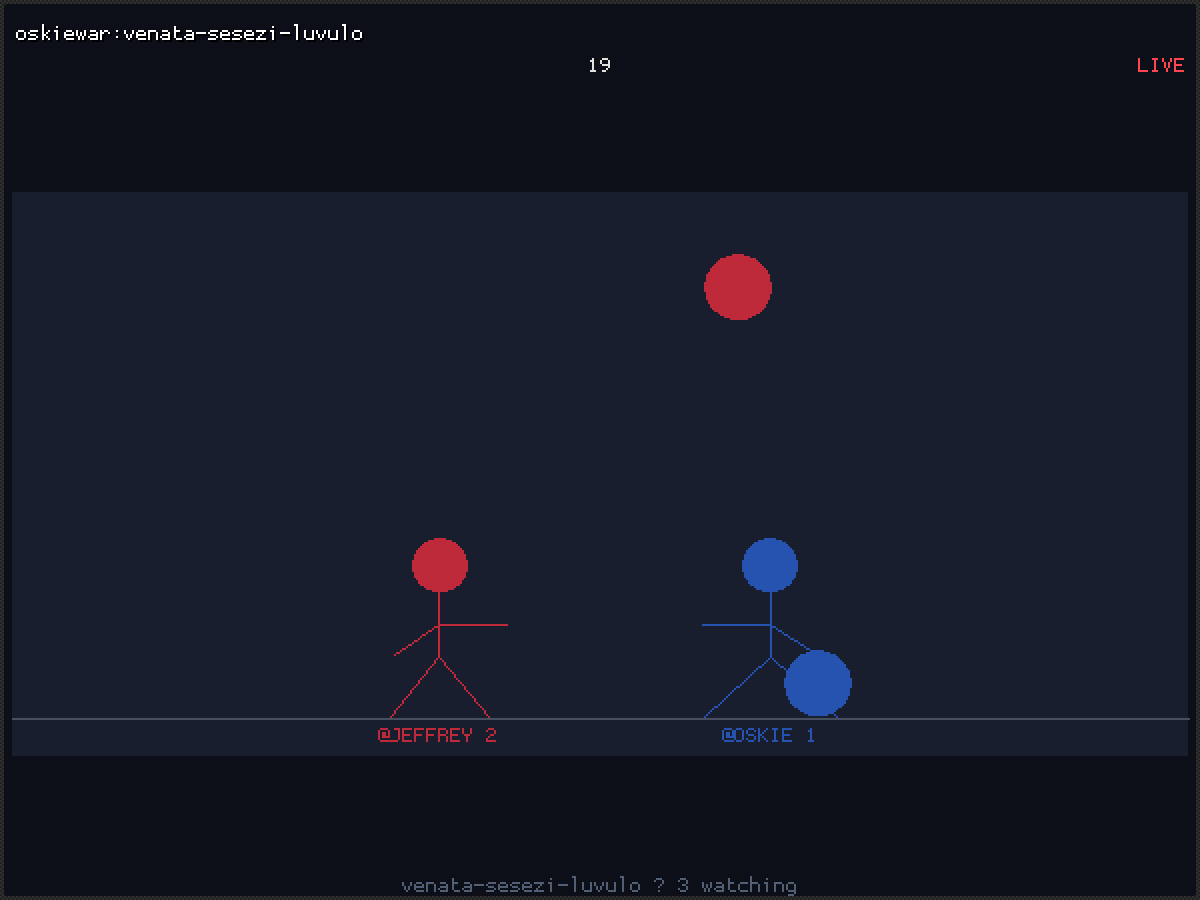
\includegraphics[width=\columnwidth]{figures/web-spectator.png}
\caption{The URL-addressable web spectator at \code{/oskiewar:venata-sesezi-luvulo}. The evidence frame uses a local schema-valid relay fixture so layout can be reproduced without a console.}
\label{fig:web-spectator}
\end{figure}

Playable web parity should not maintain a second copy of the rules. The next architecture extracts quantized commands, fixed-step simulation, collision geometry, pose state, replay serialization, and camera targets from \code{xbox/live/hello.js} into shared modules. Native and web adapters supply input, drawing, sound, persistence, and transport. Keyboard and browser gamepads map onto the same deterministic command core.

\section{Network and Capabilities}

Table~\ref{tab:endpoints} is the complete network surface used by the present build. Private console addresses and credentials are intentionally omitted. Profile endpoints are read-only enrichment; absence degrades to labels rather than blocking a match.

\begin{table*}[t]
\centering
\caption{OSKIEWAR network endpoints. Braces denote validated variables; \texttt{match} is a pronounceable three-word name and \texttt{id} is prefixed \texttt{ow-}.}
\label{tab:endpoints}
\small
\begin{tabularx}{\textwidth}{@{}p{0.19\textwidth}p{0.37\textwidth}X@{}}
\toprule
Transport & Endpoint & Capability and bound \\
\midrule
HTTPS GET & \code{https://aesthetic.computer/oskiewar:\{match\}} & Public phone spectator piece; no console address exposed.\\
WSS & \url{wss://session-server.aesthetic.computer/oskiewar-live?match=\{id\}} & Latest-only viewer stream; 64 viewers per room, 128 rooms.\\
WSS publisher & Same route with \code{\&role=publisher} & Native-only bounded publication; $\leq$7 KiB input, 20 Hz game send, 40 Hz relay ceiling.\\
HTTPS POST & \url{https://aesthetic.computer/api/oskiewar-replays} & Validated \code{ac.oskiedemo}; $\leq$512 KiB; idempotent match ID; source-hashed rate limit.\\
HTTPS GET & \code{/api/oskiewar-replays?id=\{id\}} & One full replay, or 404.\\
HTTPS GET & \code{/api/oskiewar-replays?limit=\{1..50\}} & Match count and recent replay metadata; heavy command/event arrays omitted.\\
HTTPS GET & \code{/api/clock} & Los Angeles time/theme input.\\
HTTPS GET & \code{/api/mood/moods-of-the-day} & Current handle mood/MOTD enrichment.\\
HTTPS GET & \code{/api/chat-messages?instance=clock\&limit=12} & Candidate current handle context.\\
HTTPS GET & \code{/media-collection?for=@jeffrey/painting} & Existing fighter portrait/media context.\\
HTTPS GET & \code{/api/mood/@\{handle\}} & Selected fighter MOTD.\\
HTTPS GET & \code{/api/handle-colors?handle=\{handle\}} & Per-handle identity color.\\
HTTPS GET & \url{/api/chat-messages?instance=system&limit=1&from=@\{handle\}} & Selected fighter's latest public system chat.\\
UDP outbound & broadcast \code{:51338} & OSC game signals; three copies, sequence number, queue $\leq$192.\\
UDP inbound & local \code{:51337} & Native MIDI bridge retained by the host; not required for combat input.\\
HTTPS admin & Xbox Device Portal \code{:11443} on the console's private address & Developer-Mode package install, file upload, process launch, logs, and screenshots; credentials remain outside source and this paper.\\
\bottomrule
\end{tabularx}
\end{table*}

Table~\ref{tab:capabilities} collects the user-visible system rather than repeating individual feature requests. It also marks unfinished boundaries.

\begin{table*}[t]
\centering
\caption{Current capabilities and known limits.}
\label{tab:capabilities}
\small
\begin{tabularx}{\textwidth}{@{}p{0.18\textwidth}X p{0.27\textwidth}@{}}
\toprule
Area & Implemented capability & Present limit \\
\midrule
Input & Two indexed controllers; D-pad and quantized left stick; crouch; jump; double-tap dash/ultra-jump/fast drop; disconnect clearing; input telemetry. & Visual game loop is 60 Hz in the observed build, not the requested 120 Hz.\\
Combat & Punch, kick, shield, back-block, trades, explicit stance ordering, stable pushboxes, airborne crossing, head/body/strike debug geometry. & Frame timeline, hit-stop, block-stun, action lock, buffering, and cancel windows are designed, not fully integrated.\\
World/camera & 12k bounded 3D world, floor/ceiling/walls/platform, orthographic play, perspective intros/deaths, adaptive zoom, smoothing, parallax wind. & Camera feel still requires match-scale tuning at extreme vertical separation.\\
Ball/weapons & Gravity ball; grounded boot; head-only BALLED; body bounce; shield return; cross-wack; gun/grenade pickups; diagonal fire; bullet cancellation; lethal blast/shot. & Balance values are provisional.\\
Identity/HUD & @jeffrey, @oskie, @fifi, @sat, DUMMY; handle colors; MOTD/latest-chat enrichment; compact top HUD; body-attached handles and debug state. & Remote profile data is opportunistic and may be stale or unavailable.\\
Sound & Spatial local synthesis; event OSC; Max for Live receiver; labeled sample-free Drum Rack; raw OSC bus. & UDP redundancy reduces loss but cannot mathematically guarantee delivery; receiver must observe sequence gaps.\\
Replay/spectator & Instant replay viewer; globally stored demos; match counts; public phone URL; QR; bounded latest-only relay. & Determinism across future physics versions requires migration or preservation of old simulation code.\\
Web & URL-addressable read-only spectator; interpolated fighters and balls; authoritative camera projection; live/viewer status; responsive handles beneath bodies. & Browser combat input and feature-equivalent simulation are not yet integrated.\\
Distribution & Installed name OSKIEWAR; launcher chooses OSKIEWAR or NEW GAME input lab; package 1.0.0.35. & Self-signed Developer Mode package; Microsoft Store association and certification have not been completed.\\
\bottomrule
\end{tabularx}
\end{table*}

\section{Evaluation}

The verification run on 5 August 2026 contains 49 passing checks: 41 game-client cases, six relay cases, one browser-viewer case, and one native controller-probe suite. It exercises controller indexing, axis quantization and hysteresis, tap/hold separation, disconnect reset, player-two movement, shield and back-block ordering, proximity-scaled grounded-ball blast, trades, head-only ball death, body bounce, off-camera death-shot culling, pickups, bullet cancellation, round reset, replay shape, match naming, publisher limits, viewer fan-out, malformed payload rejection, and latest-only behavior. Native preflight additionally checks JavaScript syntax, XML/package structure, portable source constraints, and the host diff.

Live telemetry from the development Xbox showed input polling work in the tens of microseconds and observed input-edge-to-present values around 12--16\,ms during a 60 Hz render loop. A later OSC snapshot reported 2,560 datagrams sent, five queued, zero dropped, and three copies per event. These are single-session operational observations, not a controlled latency distribution. They establish that the earlier large controller delay was not raw gamepad polling; stale state, dash timing, and reconciliation were the more consequential faults. Audio buffering remained roughly 52\,ms in that host session even when event-to-submit work was sub-millisecond, so sound-output latency and event transport latency must not be conflated.

One live session exposed a render failure without terminating the UWP process: a distant ball behind the orbiting death camera projected beyond the native triangle-coordinate bound. Telemetry isolated \code{RangeError: invalid triangle coordinates}; frustum culling fixed it, and a 120-frame death-camera regression now exercises the case. This distinction matters operationally: process liveness alone did not prove that the downloaded game script was still painting.

\section{Privacy, Safety, and Limits}

Spectator state is public to anyone who knows or scans the match URL. It contains game state and selected public handle labels, not controller serial numbers, console credentials, private addresses, or arbitrary chats. Profile enrichment uses already public Aesthetic Computer endpoints and should remain optional. Replay uploads hash a source network address with a server secret for rate limiting; the raw address is not stored in replay output.

The native boundary rejects oversized state and demos, validates identifiers and numeric ranges, caps queues and rooms, and does not expose arbitrary networking to the downloaded script. Device Portal remains an administrative surface on a private console address. This paper does not reproduce its credentials.

The replay format is compact but not yet a proof of deterministic portability. A versioned physics identifier prevents silent equivalence claims; long-term playback requires either retaining the corresponding simulation or migrating demos explicitly. UDP sound signals are designed for immediacy and redundant reception, not transactional certainty. Three copies plus sequence deduplication make missed hits visible and less likely, but only an acknowledged or forward-error-corrected protocol could claim stronger delivery semantics.

\section{Parallel Studies and Next Work}

Three parallel studies informed this build. The fighter-frame study produced the deterministic pose/hitbox plan summarized above. The spectator study produced and integrated the relay, viewer piece, native publisher, and QR route. A read-only Porkbun search on 4 August 2026 found \code{oskiewar.com} available and non-premium at the time of inspection; \code{oskiewar.games} was the preferred backup. Availability and prices are transient, and no domain was purchased.

The next technical sequence now begins on the web: extract one deterministic simulation and pose core; bind keyboard and browser gamepads to the existing digital command vocabulary; bring the orthographic/perspective camera and exact hit geometry into the Aesthetic Computer renderer; then reuse replay and spectator transport rather than inventing browser-only state. In parallel, the combat pulse should become fixed-frame action data; latency should be measured as distributions; the Max device should display sequence gaps; and replay runners should remain versioned. Microsoft Store association remains deferred until the account owner's authenticated review.

\section{Conclusion}

\game{} turns a controller diagnostic into a networked fighting-game instrument without abandoning the small-program character of Aesthetic Computer. Its strongest result is a portable game-state contract across a highly mutable script, a deliberately narrow console host, a bounded relay, and a URL-addressable browser piece. The native game is playable and the web spectator is operational. The next result must be deeper than another port: one deterministic combat core shared by Xbox and web, with platform-specific input, drawing, sound, and transport at its edges.

\begin{thebibliography}{9}
\bibitem{scudderPieces}
J. Scudder, ``Pieces: A Program Model for Aesthetic Computer,'' Aesthetic Computer Papers, 2026. \url{https://papers.aesthetic.computer/pieces}

\bibitem{scudderOS}
J. Scudder, ``Aesthetic Computer as an Operating System,'' Aesthetic Computer Papers, 2026. \url{https://papers.aesthetic.computer/os}

\bibitem{scudderURL}
J. Scudder, ``The URL Tradition,'' Aesthetic Computer Papers, 2026. \url{https://papers.aesthetic.computer/url-tradition}

\bibitem{scudderLatency}
J. Scudder, ``Where the Microseconds Go: Input and Audio Latency in AC Native OS,'' Aesthetic Computer Papers, 2026. \url{https://papers.aesthetic.computer/latency}

\newpage
\bibitem{scudderNotepat}
J. Scudder, ``Notepat,'' Aesthetic Computer Papers, 2026. \url{https://papers.aesthetic.computer/notepat}

\bibitem{quickjs}
F. Bellard and C. Gordon, ``QuickJS JavaScript Engine,'' 2019--2025. \url{https://bellard.org/quickjs/}

\bibitem{uwpGamepad}
Microsoft, ``Windows.Gaming.Input,'' Windows App SDK documentation. \url{https://learn.microsoft.com/uwp/api/windows.gaming.input}

\bibitem{osc}
M. Wright, ``Open Sound Control: an enabling technology for musical networking,'' Center for New Music and Audio Technologies, University of California, Berkeley, 2005.

\bibitem{repo}
Aesthetic Computer contributors, ``OSKIEWAR source, tests, native host, replay endpoint, spectator relay, web viewer, and Ableton devices,'' commits through \code{1a0a6376e0}, 5 August 2026. \url{https://github.com/whistlegraph/aesthetic-computer}
\end{thebibliography}

\end{document}
